%\begin{itemize}
%	\item adding the missing equation via a further quotient
%	\item free trace
%\end{itemize}


We now want to enforce the yanking equation on $\hide{}[\cdot]$ in $\dial C$ which is the only one
still missing to make it a trace. To do so, we follow 
the same approach as
before and further quotient $\dial C$.

\begin{definition}[trace category]
	Define the following relation on $\state C$ morphisms:
	$$\big(\,(f\monp V)\sq(B\monp\symm VV)\sq(g\monp V)\,,\, U\monp V\,\big)
	\yr V (f\sq g\,,\,U) $$
	and set $f\yl{}g=g\yr{}f$. These are then lifted to $\dial C$ morphisms by saying that two
	equivalence class are related whenever they contain two related elements.
	
	We obtain two equivalence relations:
	\begin{itemize}
		\item In $\dial C$, the transitive closure of $\yr{}\cup\yl{}$, which we write $\ye$.
		\item In $\state C$, the transitive closure of $\eq\cup\yr{}\cup\yl{}$, which we write $\quo$.
	\end{itemize}
	The \emph{trace category} over $\catf C$ is defined as $\tra C=\quotient{\dial C}{\ye}
	=\quotient{\state C}{\quo}$,
	that is the category $\dial C$ where morphisms are further equated by $\ye$ or equivalently
	the pseudo-category $\state C$ with morphisms equated by $\quo$.
\end{definition}




\begin{proposition}
	The above defined $\tra C$ is indeed a category and
	the symmetric monoidal structure of $\dial C$ lifts to $\tra C$.
\end{proposition}

\begin{proof}
	We first show that $\yr{}$ is a compatible with composition and the tensor product of $\dial C$:
	\begin{itemize}
		\item if $f\yr{}g$ then $h\sq f\yr{}h\sq g$ and $f\sq h\yr{}g\sq h$ for all suitable $h$
	\FIGURE{computation}
	\textit{(the other case is similar)}
		\item if $f\yr{}g$ then $h\otimes f\yr{}h\otimes g$ and $f\otimes h\yr{}g\otimes h$ for all $h$
	\FIGURE{computation}
	\textit{(the other case is similar)}
	\end{itemize}
	It follows from the first property that $\tra C$ is a category, and from the second that the
	$\otimes$ functor of $\dial C$ can be lifted to the equivalence classes of $\tra C$.
	Again, we need to check that we still have a monoidal structure but this time
	coherence equations and natural isomorphisms are immediately inherited from $\dial C$.
\end{proof}


	The following is obtained as the composition of the embedding of $\catf C$ into $\dial C$ and the
	quotient of $\dial C$ into $\tra C$:

\begin{proposition}
	There is a monoidal functor $\embt C$ from $\catf C$ to $\tra C$, defined as
	$\embt C(f)=(f,\unitobj)$.
\end{proposition}

%\begin{proof}
%	Because it is obtained as the composition of the embedding of $\catf C$ into $\dial C$ and the
%	quotient of $\dial C$ into $\tra C$ 
%\end{proof}

\begin{remark}
	Contrarily to the $\dial C$ case, this is not necessarily an embedding. This is actually a key
	point of this work.
\end{remark}

\begin{theorem}
	The hiding operation $\hide{}[\cdot]$ lifts to $\tra C$ and makes it a traced category.
	
	Moreover, $\tra C$ satisfies the following universal property: for any traced
	category $\catf D$ and monoidal functor $\morph F{\catf C}{\catf D}$ we have that $F$
	factors uniquely as 
	\begin{center}
	$\funcf F=\funcf G\circ \embt C$ \qquad\qquad
	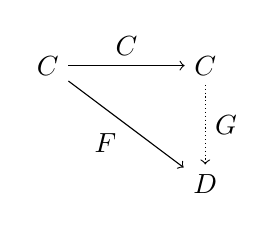
\begin{tikzpicture}[baseline=-5ex]
		\node (c) at (0,0) {$\catf C$};
		\node (tc) at (2,0) {$\tra C$};
		\node (d) at (2,-1.5) {$\catf D$};
		\draw[->] (c) to node [above] {$\embt C$} (tc);
		\draw[->] (c) to node [below left] {$\funcf F$} (d);
		\draw[->,densely dotted] (tc) to node [right] {$\funcf G$} (d);
	\end{tikzpicture}
	\end{center}
	with $G$ a traced functor.
\end{theorem}

\begin{proof}
	Similar to the proof of \autoref{th_univhiding}: define $G(f,U)=\Tr{\funcf FU}[\funcf F f]$,
	\TODO{[...]}
\end{proof}


\begin{remark}
	As before, this implies that $\tra\cdot$ is a functor. 
%	We could probably define in the same 
%	spirit an operation that takes a pseudo-traced category as an input (not necessarily the
%	result of applying $\dial\cdot$) and freely makes it a traced category.
\end{remark}

